\chapter{Design and Implementation}
\label{ch:design_implementation}

This chapter outlines the design choices and technical implementation of the delegation mechanisms introduced into the vodle platform. Each section corresponds to a key objective defined in the previous chapter, detailing how it was approached within the constraints of vodle's architecture and data model.

\section{System Architecture Overview}
Vodle is built as a serverless web application that emphasises accessibility, client-side performance, and ease of deployment. Its architecture comprises two components:

\begin{itemize}
  \item \textbf{Frontend:} Implemented using Angular and the Ionic framework, the frontend provides a responsive and modular interface that works across both desktop and mobile devices. The use of Angular facilitates the creation of component-based user interfaces, essential for introducing interactive features such as the ranked delegation UI and vote splitting sliders.
  \item \textbf{Backend:} Vodle uses CouchDB as its database. There is no custom backend logic or middleware; instead, the application communicates directly with CouchDB over HTTP. All documents, including user ratings and delegation structures, are stored in JSON format.
  \item \textbf{Implications of a serverless architecture:}
  \begin{itemize}
    \item All vote delegation logic, including transitive resolution, cycle detection, and vote splitting calculations, must be executed in the browser. This places constraints on performance and requires careful optimisation of algorithms used.
    \item The lack of a traditional server-side backend limits opportunities for centralised verification or caching, increasing the complexity of handling dynamic delegation graphs client-side.
    \item Data structures must be serialised and de-serialised as JSON, requiring careful schema design to ensure backwards compatibility and clarity across different types of delegations.
  \end{itemize}
\end{itemize}

\subsection{CouchDB overview}
% Each used remote CouchDB is identified by the URL of a CouchDB server (!) 
% (rather than the URL of a database contained in that server!).
% The CouchDB server must provide:
% - a user database named '_users' (which is the standard name for user databases)
% - a database named 'vodle' that will contain the data
% - a user named 'vodle' that has write access to both (!) these databases.
% 
% The user 'vodle' will be used by the vodle app to automatically create the other database users
% ('vodle.user.UUU', 'vodle.poll.PPP', and 'vodle.poll.PPP.voter.VVV')
% when a user logs in the first time, changes their password, creates a new poll, 
% or starts participating in a poll as a voter.
% This way the database administrator only needs to be involved when setting up the database initially,
% but not later on to create users.
% 
% Although the database user 'vodle' can create users, it cannot delete or modify users or read their passwords.
% Also, neither the database user 'vodle' or 'vodle.poll.PPP' can change their own password.
% This way, no-one can delete or overtake the database users 'vodle.user.UUU' or 'vodle.poll.PPP.voter.VVV'
% of any other person or prevent others from accessing their personal, poll, or voter data.

\section{Implement a Core Delegation Model into vodle}
\label{sec:core_delegation_detailed}

This section provides a self-contained, technical narrative of how the core delegation mechanism was conceived, which problems it solved, and how the final client-side implementation works. It follows the structure below so that each stage (from user interaction to data consistency) can be expanded or shortened independently during editing.

\subsection{Delegation Interaction Flow}
Figure~\ref{fig:delegation-flow} depicts the life-cycle of a delegation. The diagram is intentionally simple--only the four message exchanges required to set up or tear down a delegation are shown--so the reader can map each arrow to a concrete API call or UI control.

% ------------- DIAGRAM PLACEHOLDER -------------
% Replace the TikZ skeleton with an exported SVG once finalised.
\begin{figure}[H]
  \centering
  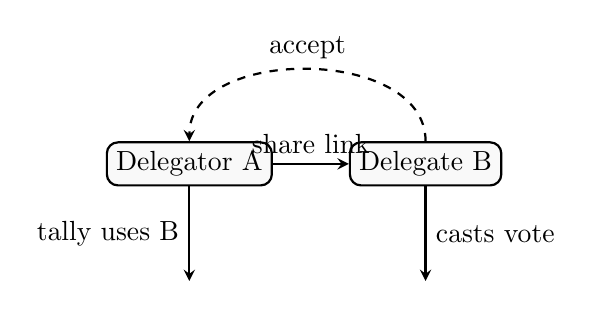
\begin{tikzpicture}[node distance=3cm,>=stealth,thick]
    % clients
    \node[rectangle,draw,rounded corners,fill=gray!5] (A) {Delegator A};
    \node[rectangle,draw,rounded corners,fill=gray!5,right of=A] (B) {Delegate B};
    % arrows
    \draw[->] (A) -- node[above]{share link} (B);
    \draw[->,dashed] (B) .. controls +(0,1.5) and +(0,1.5) .. node[above]{accept} (A);
    \draw[->] (B.south) -- ++(0,-1.2) node[midway,right]{casts vote};
    \draw[->] (A.south) -- ++(0,-1.2) node[midway,left]{tally uses B};
  \end{tikzpicture}
  \caption{Minimal message sequence for creating a delegation. Only four interactions are required: (1) A shares a link, (2) B accepts, (3) B may cast or delegate further, (4) A's vote resolves through B.}
  \label{fig:delegation-flow}
\end{figure}

At runtime the app must therefore support:
\begin{enumerate}
  \item Generating and copying a poll-scoped, user-scoped invitation link.
  \item Polling CouchDB for acceptance (or rejection) of that link.
  \item A client-side resolution routine that follows the chain of \texttt{delegateFor} relationships until a casting voter is found.
  \item Revocation that is immediate yet conflict-free if multiple clients are open.
\end{enumerate}

\subsection{Current Issues Prior to Redesign}
\begin{description}
  \item[Out-of-sync state] Each browser session cached its own copy of the delegation graph; no push notifications existed to bring other clients up-to-date.
  \item[Inconsistent cycle checking] Because state diverged, the local "no-loop" tests sometimes produced different answers on different machines.
  \item[UI drift] Controls such as ``delegate none/some/all'' and the ``your vote is used for \(n\) others'' badge used stale data and became misleading.
\end{description}

\subsection{Cycle Checking}
The following section details the design and implementation of a cycle-checking algorithm that was added to the core delegation model as well as the data structures and synchronisation mechanisms that were introduced to support it.
\subsubsection{Algorithm Design}
The current delegations in a system can be represented as a directed graph where each user is represented as a node and each delegation is represented as a directed edge $(u,v)$, where $u$ is the delegator and $v$ is the delegate. The goal of the cycle-checking algorithm is to ensure that a proposed delegation does not create a cycle in this directed graph.

A new delegation $X\to Y$ is valid if and only if $Y$ is \emph{not} reachable from $X$ in that DAG -- if $Y$ is not a descendant of $X$.

Instead of checking for this condition directly using a depth-first search (DFS) or breadth-first search (BFS), a more efficient approach is to maintain a list of all descendants for each user. This allows us to check if $Y$ is in the list of descendants of $X$ in constant time. This implementation will be detailed in the following section.

\subsubsection{Implementation Details}
A hashmap is used to store the descendants of each user. The keys are user IDs, and the values are sets of user IDs representing the direct delegates of that user. In the code, this hashmap is referred to as ``\verb|inverse_indirect_map|''.
\begin{figure}[H]
  \centering
  \begin{minted}{json}
    "inverse_indirect_map": {
      "B": ["A"],
      "C": ["B", "A"],
      "D": ["C", "B", "A"]
    }
  \end{minted}
  \caption{Example of a hashmap for users A, B, C, and D. User A has delegated to B, user B has delegated to C, and user C has delegated to D. Consequently, the descendants of user D are A, B and C.}
  \label{fig:inverse_indirect_map}
\end{figure}

This structure allows for the following operations:
\paragraph{Check Delegation} To check if a delegation \(X\!\to\!Y\) is valid, we simply check if \(Y\) is in the set of descendants of \(X\). This operation takes \(O(1)\) time.
\begin{figure}[H]
  \centering
  \begin{minted}{javascript}
    const inverse_indirect_map = this.G.D.get_inverse_indirect_map(pid);
    const descendant_set = inverse_indirect_map.get(delegate_vid);
    if (descendant_set.has(myvid)) {
      cycle = true;
    }
  \end{minted}
  \caption{Code for checking if a delegation is valid. This check is done when a user clicks on a delegate link. The map is retrieved from the synced local cache, and the set of descendants for the delegator is checked to see if it contains the current user.}
\end{figure}


\begin{itemize}
  \item \textbf{Check Delegation}: to decide if \(X\!\to\!Y\) is legal, verify that \verb|Y| $\notin$ \verb|map[X]| (\(O(1)\)).
  \item \textbf{Add Edge}: \verb|map[Y]| $\leftarrow$ \verb|map[Y]| $\cup$ \verb|map[X]| $\cup$ \{\verb|X|\}.
  \item \textbf{Remove Edge}: \verb|map[Y]| $\leftarrow$ \verb|map[Y]| \textbackslash{} (\verb|map[X]| $\cup$ \{\verb|X|\}). Because the graph is a DAG, it is not possible for the descendants of $X$ to be a subset of the descendants of $Y$ after removing the edge $X\to Y$.
\end{itemize}

\paragraph{Persistence} The map lives alongside the poll document so every client shares one authoritative copy. Although ordinary poll docs are append-only, a special admin rule now allows updates at the key \verb|inverse_indirect_map|. Conflict fields (\verb|_rev| in CouchDB) ensure last-write-wins semantics while we serialise edits.

\subsubsection{Practical Challenges}
\begin{itemize}
  \item blank 4 now.
\end{itemize}

\subsection{UI Fixes}
\begin{itemize}
  \item Re-bound the ``delegate none/some/all'' switch so it toggles \emph{only} the current option and refreshes its label after server confirmation.
  \item Re-implemented the ``vote is used for \(n\) others'' badge so it recomputes from the latest \texttt{inverse\_indirect\_map} rather than client guesses.
  \item Added unobtrusive toast notifications when a delegation request is rejected (e.g.\ cycle detected) so the user can immediately choose another delegate.
\end{itemize}

\subsection{Summary}
The redesign introduced a lightweight yet provably correct cycle-checking algorithm, synchronised across clients by persisting an \texttt{inverse\_indirect\_map} in the poll document. Combined with targeted UI fixes, the core delegation model now (i) prevents loops, (ii) reflects state consistently across devices, and (iii) scales to thousands of voters without central servers.


\section{Implement Ranked Delegation into Vodle}
This feature introduced ranked delegation using the MinSum rule, allowing users to list fallback delegates in case their primary choice was unavailable.

\begin{itemize}
  \item UI for setting delegate rankings
  \item \verb|direct_delegation_map|: maps user IDs to list of ranked delegates [[delegationid, rank, status]...]
  \item Explanation and application of the MinSum rule
  \item Implementation of ranked path resolution
  \item Illustrations and code snippets
\end{itemize}

\subsubsection{Challenges}
The MinSum rule had to be implemented efficiently using only browser-based resources. Ranking resolution had to preserve user intent while avoiding delegation ambiguity. Providing visual feedback to help users understand how rankings would resolve added an additional layer of design complexity.

\section{Implement a Vote Splitting Delegation Mechanism into Vodle}
Vote splitting was implemented to allow users to distribute fractional influence to multiple delegates.

\begin{itemize}
  \item UI for assigning weights
  \item modify\verb|direct_delegation_map|to include weights [[delegationid, weight, status]...]
  \item Computation of weighted vote outcomes
  \item Constraints:
  \begin{itemize}
    \item Weight sum limit (\texttt{< 1.0})
    \item Error handling
  \end{itemize}
  \item Algorithm integration and frontend testing
\end{itemize}

\subsubsection{Challenges}
The vote splitting logic needed to maintain consistency with the MaxParC aggregation model, while ensuring intuitive user experience. Edge cases (e.g., partially overlapping delegate chains or missing data) introduced complexity during testing. Rendering weight distributions clearly in the UI while keeping the interface lightweight was a recurring challenge.

\section{Implement the Ability to Delegate Individual Options to Different Users}
This feature enabled per-option delegation, allowing users to assign a different delegate for each item in a poll.

\begin{itemize}
  \item Per-option delegate selection interface
  \item Independent resolution of each delegated option
  \item talk about nested map - need to take care to serialise.
  \item \verb|direct_delegation_map|: \verb|option_id| -> \verb|user_id| -> [delegationid, null, status]
  \item \verb|inverse_indirect_map|: \verb|option_id| -> \verb|user_id| -> list of users who have delegated to them, either directly or indirectly.
  \item Storage schema modifications
\end{itemize}

\subsubsection{Challenges}
This mechanism required updates to the internal delegation logic to handle resolution at the option level. The user interface also had to be adapted to display multiple concurrent delegate selections without overwhelming the user. Debugging resolution logic for hybrid delegation modes (e.g., one direct, one split, one ranked) was non-trivial.

\section{Simulate Delegation Mechanisms}
The simulation objective was de-scoped due to time constraints and prioritisation of implementation work. While initial planning and framework selection (Mesa) were completed, no functional simulation code was delivered. The decision to drop this extension is discussed further in the Project Management chapter.

\section{Design Decisions and Trade-offs}
\begin{itemize}
  \item All logic had to run client-side due to the serverless CouchDB architecture, limiting complexity and computational resources.
  \item A consistent JSON format was required for all data models, impacting flexibility in data design.
  \item Trade-offs were made between expressive delegation types and usability, particularly in the option-specific and vote splitting interfaces.
\end{itemize}

\section{Summary}
\begin{itemize}
  \item Each objective was successfully implemented within the constraints of the vodle platform.
  \item Challenges were primarily technical (client-side performance, real-time resolution) and design-oriented (clarity and control for users).
  \item The final implementation offers a modular, extensible delegation system that addresses the key theoretical and practical limitations outlined in earlier chapters.
\end{itemize}

